\chapter{Second and Third Trajectory}
The second trajectory to complete the task seen in \autoref{fig:secondTask} is different than the first, in that it does not require movement in the ($\theta$, $\dot{\theta}$)-plane, in fact, rather the contrary. It does however require the cart to move forward in order to pass the obstacles and hold up the pendulum.\\
As before, the initial values are known and a final position of the cart can be chosen, which will be the condition for switching to the final task.\\
Substituting the initial and final values, $\theta = \theta_\mathrm{f}$, $\dot{\theta} = 0$ and $\ddot{\theta} = 0$, into \autoref{eq:dynamicEquationsNoFriction}, reduces the dynamics to,
%
\begin{flalign}
  \begin{cases}
    - m l \cos \theta_\mathrm{f} \ddot{x} - m g l \sin \theta_\mathrm{f}  = 0  & \\                      %\unit{N \cdot m}  \\
    ( M + m )\ddot{x}  =  F  \ \ \ . &   %\unit{N \cdot m}
  \end{cases} & \unit{\cdot}
  \label{eq:dynamicEquation2SecondTrajectory}
\end{flalign}
%
In \autoref{eq:dynamicEquation2SecondTrajectory} the force, $F$, is directly provided as a function of the acceleration of the cart. Feeding back $\ddot{x}$ in this manner will attempt to keep the angle of the pendulum steady while moving forward through the obstacles.
%It is interesting to note that the average of the force excreted during this second trajectory changes the $\theta$-dynamics in such a way that the angle and angular velocity are kept in a saddle point equilibrium.
%%
%\begin{figure}[H]
%  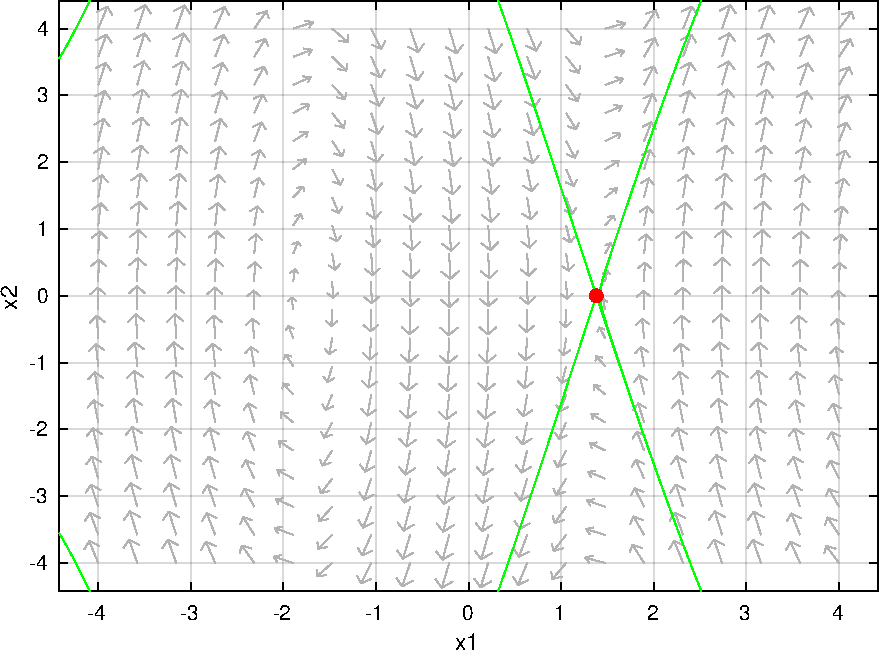
\includegraphics[width=.6\textwidth]{figures/secondTrajectory}
%  \caption{Phase portrait showing how the $\theta$-dynamics changes given a constant force averaged from the forces used during the second trajectory. The system is kept near the indicated saddle point equilibrium.}
%  \label{fig:phasePortraitSecondTrajectory}
%\end{figure}

For the third and final trajectory, the idea is to stop the system. This is achieved using \autoref{eq:alphaBetaGammaYPQintFactorProductRuleIntegrationGeneralPQbackLimitsPsi_pendulum}, where $(\theta_0,\dot{\theta}_0) = ( \frac{7\pi}{8} , 0 )$ and the final values, $(\theta,\dot{\theta} = ( \pi , 0 )$. While this does bring the pendulum to rest, the cart still has momentum and will drag the pendulum out of equilibrium after which the system is caught in a stable orbit since there is no friction to dampen the oscillations. This issue was not solved during this project.
